\documentclass{article}

%% Language and font encodings
\usepackage[english]{babel}
\usepackage[utf8x]{inputenc}
\usepackage[T1]{fontenc}

%% Sets page size and margins
\usepackage[a4paper,top=3cm,bottom=2cm,left=3cm,right=3cm,marginparwidth=1.75cm]{geometry}

%% Useful packages
\usepackage{amsmath}
\usepackage{graphicx}
\usepackage[colorinlistoftodos]{todonotes}
\usepackage[colorlinks=true, allcolors=blue]{hyperref}

\title{SVM report}

\begin{document}
\maketitle

\section{Introduction}
The project is aimed at building a more effective recommendation system. Through this system, Santander can predict which products their existing customers will buy in the next month based on their past behavior and that of similar customers. Under Santander Bank current system, the recommendations cannot meet the individual needs well. It is necessary to apply machine learning methods to improve the recommendations system. One of the difficulties is how to deal with the large data set. Indeed, the original data set contains 13 million records from January 2015 to June 2016, with approximate 930 thousand customers. How to deal with the large data set and transform the data to the model are the core problems of this project.

In our project, we applied four methods to solve this prediction problem: logistic regression, random forest, SVM and xgboost. For each method, the ways to clean and process the data are different but there are still some similarity.
For instance, we dropped some variables which are not important to the prediction issue. Besides, we converted some complicated features to a understandable form, in order to simplify the model. Within each method, we tuned parameters and several models and chose one with the best performance. After fitting the model, we evaluated the performance of the four methods and got final conclusion.

This paper introduces four machine learning methods. In each sub parts, we will introduce the way we clean the data, models and results, and the discussions of this method.

\section{Methods}

\subsection{Process the data}
\begin{enumerate}
\item Independent Variable Selection

In order to increase the accuracy of model and efficiency of calculation, remove should remove some independent variables:

\begin{itemize}
\item Since we should transform categorical variables into dummy variables, variables(canal\_ entrada) with too many levels would sharply increase the model complexity and decrease the effectiveness of calculation.

\item We also leave out independent variables that have repeated information. For example, indresi(whether residence country is the same as the bank country) and nomprov(i.e Province name) reflect the similar information of the customer so we could only keep one of them. 

\item For the independent variables predominated by missing values,such as conyuemp, we leave them out because they could not reflect useful information. 
\end{itemize}

According to these three  rules, we remove : pais\_residencia, fecha\_alta, indext, conyuemp, canal\_entrada, tipodom, cod\_prov and nomprov. 

\item  Missing values

For the cases have missing values in any of the 24 dependent variables, we remove them for the reason that these missing values only proportion less than 1\% and did not show no obvious pattern. 

As for independent variables, we only find missing values in renta(gross income), we use the regional average to replace the missing values. 

\item Data Transformation

For independent variables, we transform the categorical variables into dummy variable. For the variable with n levels, we create (n-1) dummy variables. Besides, aimed to avoid influence of units and scales, we standardize the continuous variables. 

Then we process the response variables.  Owing that our goal is to predict what additional products a customer will get in addition to what they already have at the last month. So the value of the next month minus that of the current month.  If the result is “1”, we could figure out the customer bought certain new product i. Otherwise The consumer did not buy new products. 

Thus, we could build model to predict additional products consumers would buy for next month given their personal characteristics and their consumption records at current month.
\end{enumerate}

\subsection{SVM Model}

Support vector machine (i.e SVM) is the supervised learning model that analyze the data used for classification. With associated learning algorithms, a line or a hyper-plane is found to classify the data. In addition to doing linear classification, SVM can also efficiently perform a non-linear classification using kernel, making the separating hyper-plane complicated and do the classification better.

In our case, we want the classifier to be less sensitive to outliers to keep the margin sufficiently large. To do so, we introduce “slack variables” that allow samples to be misclassified or be within the margin. Additionally, to make the samples more separable, we introduce the idea of kernel. Consequently, we have :

Decision function:
$$f(x) = \displaystyle\sum_{i}\alpha_i\Phi(x_i)\Phi(x)+b = \displaystyle\sum_{i}\alpha_{i} K(x_i, x)+b$$, where $K(x_i, x)$ is the Kernel function.

Dual formulation:
$$min P(w,b) = \frac{1}{2}(||\displaystyle\sum_{i=1}^{m}\alpha_i\Phi(x_i)||)^2 + C\displaystyle\sum_{i}H_{i}[y_{i}f(x_i)]$$

\section{Results}

Based on the result of SVM and real labels of the 24 dependent variables, we calculate accuracy for each estimation. Namely:
$$Accuracy = \frac{TP+TN}{P+N}$$
Where TP is count of true positive , TN is count of true negative , N is count of negative and P is count of positive.

We found that, for each of the 24 estimation, the accuracy is higher than 99\% which indicates a high performance of the model in predicting each single dependent variable.

The we calculate the overall accuracy:
$$Overall\enspace Accuracy = \frac{Counts\enspace of\enspace the\enspace cases\enspace which\enspace all\enspace the\enspace 24\enspace variables\enspace are\enspace predicted\enspace correctly}{total\enspace number\enspace of\enspace cases}$$
In this case, the overall accuracy rate is 98\% which shows SVM method accuate result.

\section{Discussion}

However, scuritiny of the data reveals simply focusing on the accuracy is not reasonable. Precisely, for most dependent variables, the negative class 0 is predominant (typically greater than 99\%). Thus, even though all the predictions are zeros, the accuracy would be still easily over 99\%, based on which, the high performance might be caused by the fact that wrong prediction in 1s does not have much influence on the accuracy. To examine this idea, we choose 3 different dependent variables, each of which has very asymmetric distribution in 0s and 1s, and then use ROC and PRC to exhibit the results:

$$True\enspace Positive\enspace Rate = Recall = \frac{TP}{TP+FN}, Precision = \frac{TP}{TP+FP}$$

In the following plots, we can observe when the negative class 0 is highly predominant, the ROC and PRC suggest our results are actually problematic despite the fact that the accuracys are pretty good. Below is the confusion matrix for response variable "ind\_cco\_fin\_ult1".

\vspace{5mm}
\begin{tabular}{| l | l | l |}
\hline
  & Really True & Really False \\ \hline
Predicted True & 0 & 0 \\ \hline
Predicted False & 558 & 99442\\
\hline
\end{tabular}
\vspace{5mm}

The accuracy here is really high only, which is 99.44\%. However the model is completely useless since we are very interested in helping the bank to recommend products to a potential customer in addition to what he/she already has. Thus, it is very important to correctly classify 1 as 1. Failing to consider other metrics of evaluation like precision and recall would lead to an unjustified model. Here the recall is 0 and the precision is NA because there is not a single observation being classified as 1. The reason for this is that the negative class 0 is predominant in "ind\_cco\_fin\_ult1" and the model tends to classify everything as 0, producing that all the 1’s are classified as 0. The results are even worse for the other two variables as the class 1 are fewer.

ROC and PRC curve for "ind\_cco\_fin\_ult1" , "ind\_fond\_fin\_ult1" and "ind\_deme\_fin\_ult1" 

\vspace{5mm}
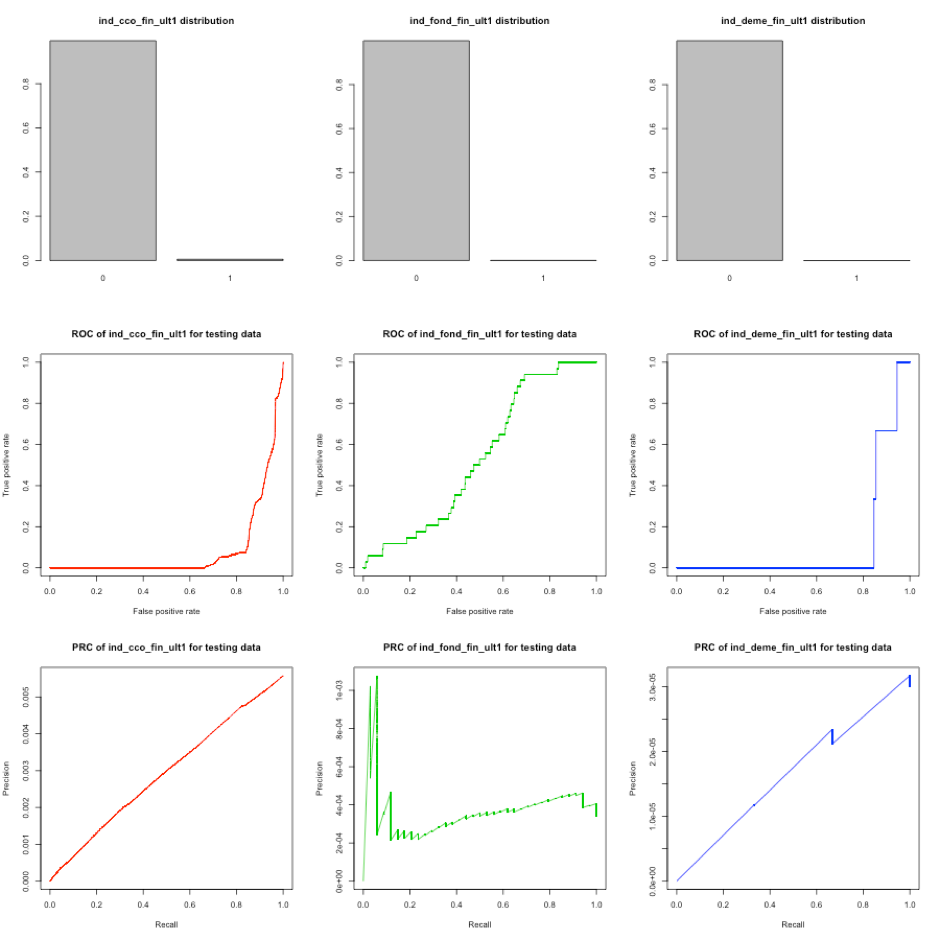
\includegraphics[scale = 0.8]{ROCandPR.png}
\vspace{5mm}

We come up with two solutions to deal with this skewed class problem. One is to replace random sampling for training set and testing data by stratified sampling, which assures that the training set and testing data are well balanced. Random sampling seems to be reasonable but in our case, class 1 is really scarce. Therefore it is likely that all those class 1 being sampled into testing set, which makes it impossible for our algorithm to learn the hidden pattern of class 1. The other workaround is to add higher weights to the minority class which would encourage the model to be gear towards classifying 1 as 1 and add some penalty for model to predict 0. We tried the second option by adding weights to the two classes which are inverse proportional to their fractions. The results are as follows. It is shown that all class 1’s are correctly classified! Now the precision and recall are 1.64\% and 100\%. But there is some inevitable trade offs as in general one of these two metric gets better, the other will get worse. Additionally, since we add more penalty when the model predicts 0, there are plenty of class 0 being misclassified which leads to accuracy decreasing to 66.51 as well as decreasing in specifity. However, in our case, recall should be the first priority as we do not want to lose any potential customers, we should accept this trade off. It is also worth noting that another downside is that the process for training model is more time consuming than before.

\vspace{5mm}
\begin{tabular}{| l | l | l |}
\hline
  & Really True & Really False \\ \hline
Predicted True & 558 & 33488 \\ \hline
Predicted False & 0 & 65954\\
\hline
\end{tabular}
\vspace{5mm}

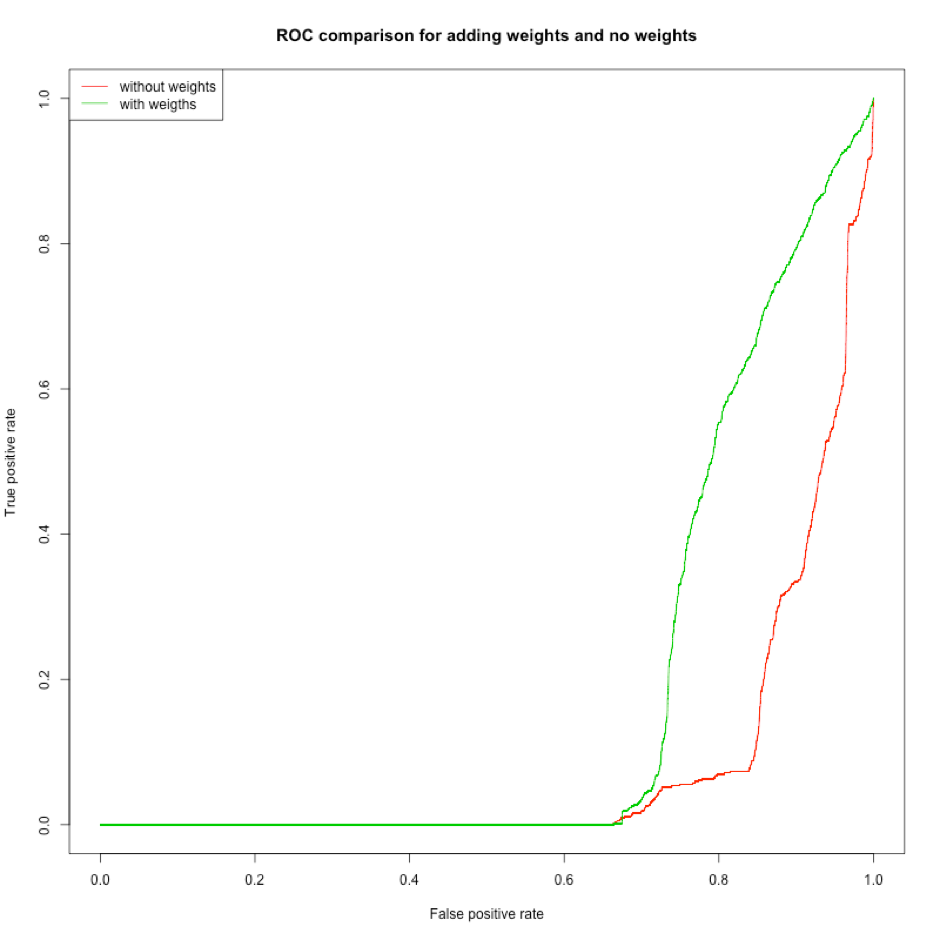
\includegraphics[scale = 0.8]{ROCwithandwithoutweights.png}

\begin{thebibliography}{9}
\bibitem{book}
Gareth James, Daniela Witten, Trevor Hastie, Robert Tibshirani, \textit{An Introduction to Statistical Learning}. New York, USA: Springer, 2013.
\bibitem{book}
Trevor Hastie, Robert Tibshirani, Jerome Friedman, \textit{The Elements of Statistical Learning}. New York, USA: Springer, 2008.
\bibitem{Amlbook}
Yaser S. Abu-Mosta, Malik Magdon-Ismail, Hsuan-Tien Lin, \textit{Learning From Data: A Short Course}. New York, USA: AMLBook, 2012.
\bibitem{book}Kevin, P. Murphy, \textit{Machine Learning: A Probabilistic Perspective}. London, England:The MIT Press, Cambridge Massachusetts, 2012.
\bibitem{paper}
herkassky, Vladimir, and Yunqian Ma, \textit{Practical selection of SVM parameters and noise estimation for SVM regression}. Neural networks 17.1 (2004): 113-126.

\end{thebibliography}

\section{Author contributions}
\begin{enumerate}
\item
Data processing:Aoran Zhang, Huiyu Bi
\item
Data analysis and interpretation: Meng Li, Zhongyu Fan, Huiyu Bi
\item
Model analysis and interpretation:Aoran Zhang, Meng Li
\item
Drafting the article: Aoran Zhang, Meng Li, Huiyu Bi, Zhongyu Fan
\item
Critical revision of the article:Aoran Zhang, Zhongyu Fan

\end{enumerate}

\end{document}


